\documentclass[14pt]{extbook}
\usepackage{multicol, enumerate, enumitem, hyperref, color, soul, setspace, parskip, fancyhdr} %General Packages
\usepackage{amssymb, amsthm, amsmath, bbm, latexsym, units, mathtools} %Math Packages
\everymath{\displaystyle} %All math in Display Style
% Packages with additional options
\usepackage[headsep=0.5cm,headheight=12pt, left=1 in,right= 1 in,top= 1 in,bottom= 1 in]{geometry}
\usepackage[usenames,dvipsnames]{xcolor}
\usepackage{dashrule}  % Package to use the command below to create lines between items
\newcommand{\litem}[1]{\item#1\hspace*{-1cm}\rule{\textwidth}{0.4pt}}
\pagestyle{fancy}
\lhead{Makeup Progress Quiz -1}
\chead{}
\rhead{Version C}
\lfoot{7547-2949}
\cfoot{}
\rfoot{Fall 2020}
\begin{document}

\begin{enumerate}
\litem{
Solve the quadratic equation below. Then, choose the intervals that the solutions belong to, with $x_1 \leq x_2$ (if they exist).\[ -11x^{2} -12 x + 8 = 0 \]\begin{enumerate}[label=\Alph*.]
\item \( x_1 \in [-0.47, 2.53] \text{ and } x_2 \in [1.1, 3] \)
\item \( x_1 \in [-6.14, -3.14] \text{ and } x_2 \in [15.4, 18.6] \)
\item \( x_1 \in [-1.56, -0.56] \text{ and } x_2 \in [-1, 1.5] \)
\item \( x_1 \in [-25.82, -19.82] \text{ and } x_2 \in [21, 23.4] \)
\item \( \text{There are no Real solutions.} \)

\end{enumerate} }
\litem{
Graph the equation below.\[ f(x) = (x-2)^2 - 14 \]\begin{enumerate}[label=\Alph*.]
\begin{multicols}{2}\item 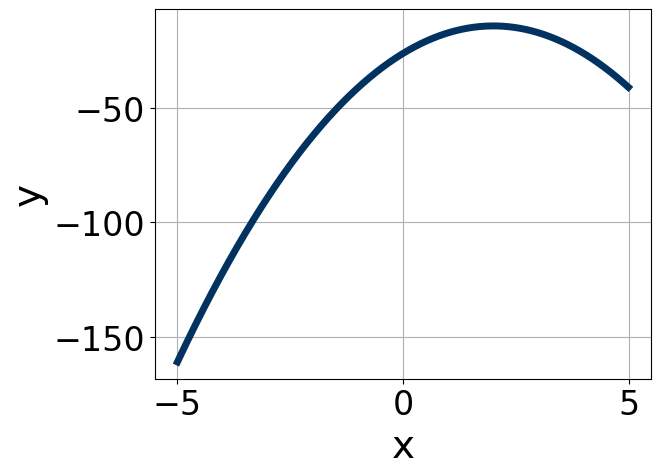
\includegraphics[width = 0.3\textwidth]{../Figures/quadraticEquationToGraphCopyAC.png}\item 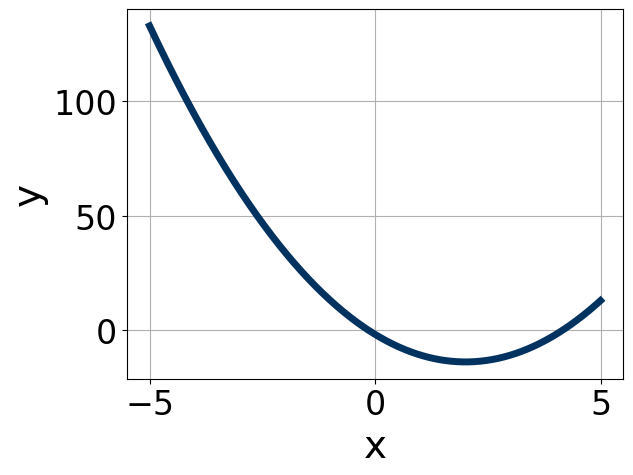
\includegraphics[width = 0.3\textwidth]{../Figures/quadraticEquationToGraphCopyBC.png}\item 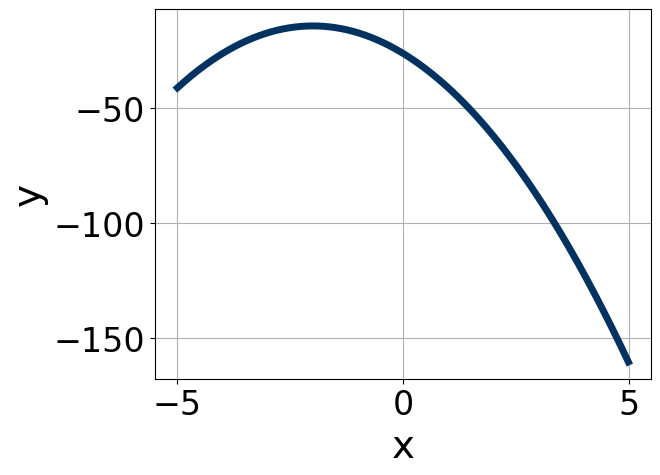
\includegraphics[width = 0.3\textwidth]{../Figures/quadraticEquationToGraphCopyCC.png}\item 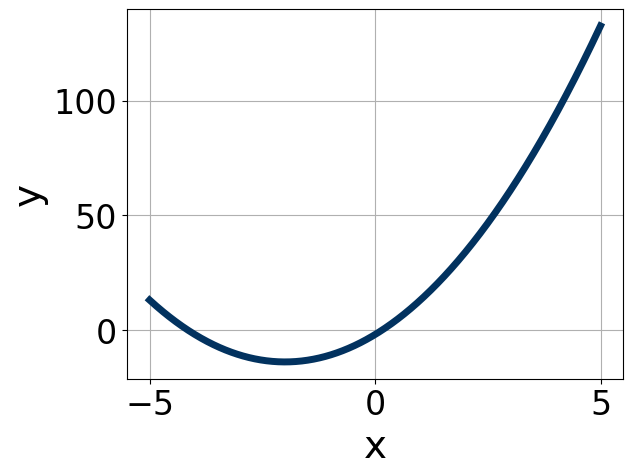
\includegraphics[width = 0.3\textwidth]{../Figures/quadraticEquationToGraphCopyDC.png}\end{multicols}\item None of the above.
\end{enumerate} }
\litem{
Graph the equation below.\[ f(x) = (x-2)^2 + 13 \]\begin{enumerate}[label=\Alph*.]
\begin{multicols}{2}\item 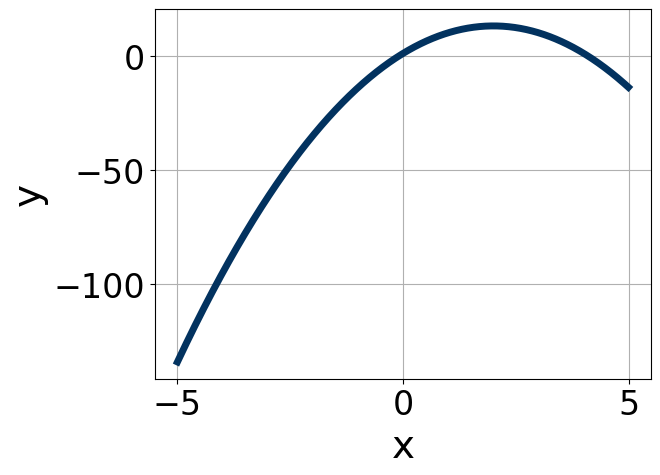
\includegraphics[width = 0.3\textwidth]{../Figures/quadraticEquationToGraphAC.png}\item 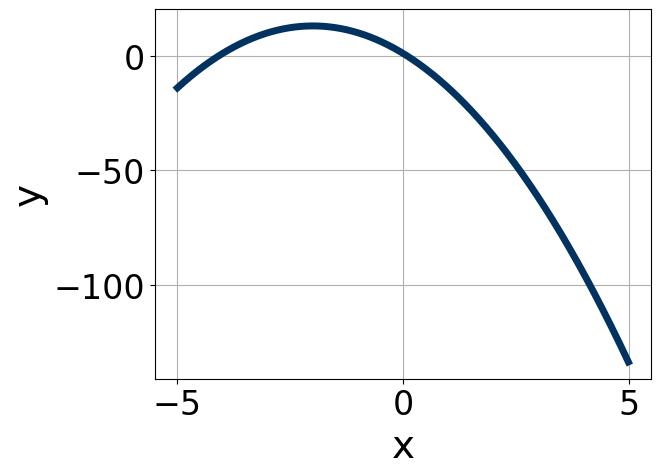
\includegraphics[width = 0.3\textwidth]{../Figures/quadraticEquationToGraphBC.png}\item 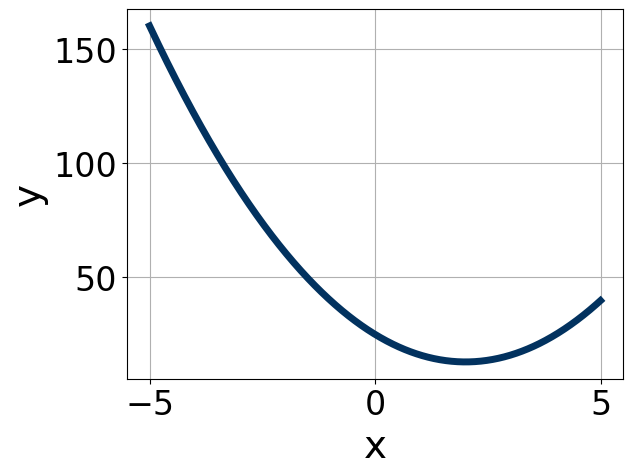
\includegraphics[width = 0.3\textwidth]{../Figures/quadraticEquationToGraphCC.png}\item 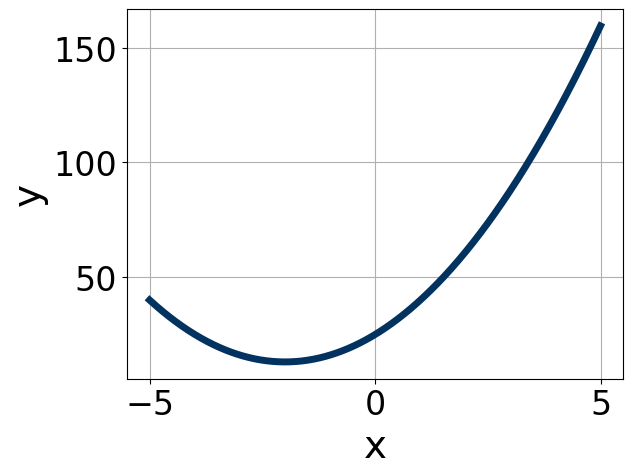
\includegraphics[width = 0.3\textwidth]{../Figures/quadraticEquationToGraphDC.png}\end{multicols}\item None of the above.
\end{enumerate} }
\litem{
Solve the quadratic equation below. Then, choose the intervals that the solutions $x_1$ and $x_2$ belong to, with $x_1 \leq x_2$.\[ 25x^{2} -15 x -54 = 0 \]\begin{enumerate}[label=\Alph*.]
\item \( x_1 \in [-31.56, -29.87] \text{ and } x_2 \in [44.88, 45.74] \)
\item \( x_1 \in [-6.24, -5.89] \text{ and } x_2 \in [-0.18, 0.58] \)
\item \( x_1 \in [-4.81, -2.99] \text{ and } x_2 \in [0.43, 1.43] \)
\item \( x_1 \in [-0.66, 0.75] \text{ and } x_2 \in [3.07, 4.1] \)
\item \( x_1 \in [-2.23, -0.95] \text{ and } x_2 \in [1.33, 1.92] \)

\end{enumerate} }
\litem{
Write the equation of the graph presented below in the form $f(x)=ax^2+bx+c$, assuming  $a=1$ or $a=-1$. Then, choose the intervals that $a, b,$ and $c$ belong to.
\begin{center}
    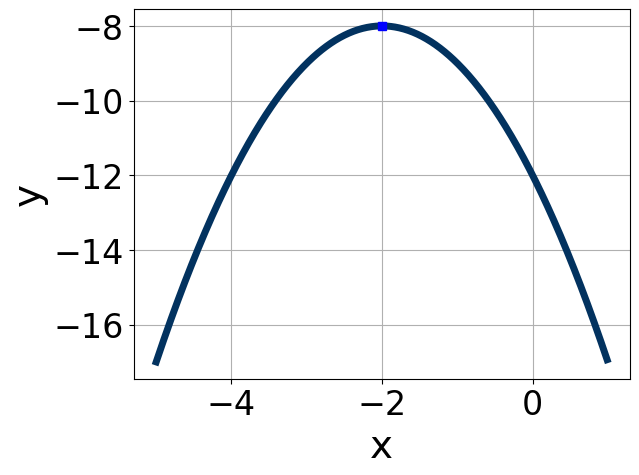
\includegraphics[width=0.5\textwidth]{../Figures/quadraticGraphToEquationCopyC.png}
\end{center}
\begin{enumerate}[label=\Alph*.]
\item \( a \in [1, 3], \hspace*{5mm} b \in [3, 7], \text{ and } \hspace*{5mm} c \in [-7, 1] \)
\item \( a \in [-3, 0], \hspace*{5mm} b \in [3, 7], \text{ and } \hspace*{5mm} c \in [4, 7] \)
\item \( a \in [-3, 0], \hspace*{5mm} b \in [3, 7], \text{ and } \hspace*{5mm} c \in [-12, -11] \)
\item \( a \in [1, 3], \hspace*{5mm} b \in [-6, -1], \text{ and } \hspace*{5mm} c \in [-7, 1] \)
\item \( a \in [-3, 0], \hspace*{5mm} b \in [-6, -1], \text{ and } \hspace*{5mm} c \in [-12, -11] \)

\end{enumerate} }
\litem{
Factor the quadratic below. Then, choose the intervals that contain the constants in the form $(ax+b)(cx+d); b \leq d.$\[ 54x^{2} +75 x + 25 \]\begin{enumerate}[label=\Alph*.]
\item \( a \in [5.3, 8.7], \hspace*{5mm} b \in [4, 7], \hspace*{5mm} c \in [8.35, 9.98], \text{ and } \hspace*{5mm} d \in [2, 7] \)
\item \( a \in [15.9, 20], \hspace*{5mm} b \in [4, 7], \hspace*{5mm} c \in [1.64, 3.11], \text{ and } \hspace*{5mm} d \in [2, 7] \)
\item \( a \in [0.5, 2.3], \hspace*{5mm} b \in [26, 35], \hspace*{5mm} c \in [-0.06, 1.12], \text{ and } \hspace*{5mm} d \in [45, 46] \)
\item \( a \in [2.3, 3.6], \hspace*{5mm} b \in [4, 7], \hspace*{5mm} c \in [16.26, 18.25], \text{ and } \hspace*{5mm} d \in [2, 7] \)
\item \( \text{None of the above.} \)

\end{enumerate} }
\litem{
Solve the quadratic equation below. Then, choose the intervals that the solutions $x_1$ and $x_2$ belong to, with $x_1 \leq x_2$.\[ 25x^{2} +60 x + 36 = 0 \]\begin{enumerate}[label=\Alph*.]
\item \( x_1 \in [-6.9, -4.15] \text{ and } x_2 \in [-0.26, -0.22] \)
\item \( x_1 \in [-2.11, 0.81] \text{ and } x_2 \in [-1.45, -0.96] \)
\item \( x_1 \in [-3.84, -2.54] \text{ and } x_2 \in [-0.57, -0.37] \)
\item \( x_1 \in [-3.18, -2.11] \text{ and } x_2 \in [-0.82, -0.53] \)
\item \( x_1 \in [-30.31, -29.48] \text{ and } x_2 \in [-30.07, -29.91] \)

\end{enumerate} }
\litem{
Factor the quadratic below. Then, choose the intervals that contain the constants in the form $(ax+b)(cx+d); b \leq d.$\[ 36x^{2} +60 x + 25 \]\begin{enumerate}[label=\Alph*.]
\item \( a \in [11.2, 15.4], \hspace*{5mm} b \in [1, 7], \hspace*{5mm} c \in [2.5, 4.7], \text{ and } \hspace*{5mm} d \in [4, 7] \)
\item \( a \in [-0.7, 2], \hspace*{5mm} b \in [24, 32], \hspace*{5mm} c \in [-0.3, 2], \text{ and } \hspace*{5mm} d \in [24, 32] \)
\item \( a \in [5.4, 7.1], \hspace*{5mm} b \in [1, 7], \hspace*{5mm} c \in [5.7, 8.3], \text{ and } \hspace*{5mm} d \in [4, 7] \)
\item \( a \in [2.5, 3.3], \hspace*{5mm} b \in [1, 7], \hspace*{5mm} c \in [10, 13.1], \text{ and } \hspace*{5mm} d \in [4, 7] \)
\item \( \text{None of the above.} \)

\end{enumerate} }
\litem{
Solve the quadratic equation below. Then, choose the intervals that the solutions belong to, with $x_1 \leq x_2$ (if they exist).\[ -17x^{2} -13 x + 9 = 0 \]\begin{enumerate}[label=\Alph*.]
\item \( x_1 \in [-2.8, -0.5] \text{ and } x_2 \in [-1.4, 0.9] \)
\item \( x_1 \in [-0.9, 2.6] \text{ and } x_2 \in [0.7, 2.3] \)
\item \( x_1 \in [-29.4, -27.3] \text{ and } x_2 \in [25.8, 27.9] \)
\item \( x_1 \in [-9.1, -5.5] \text{ and } x_2 \in [18.3, 20.8] \)
\item \( \text{There are no Real solutions.} \)

\end{enumerate} }
\litem{
Write the equation of the graph presented below in the form $f(x)=ax^2+bx+c$, assuming  $a=1$ or $a=-1$. Then, choose the intervals that $a, b,$ and $c$ belong to.
\begin{center}
    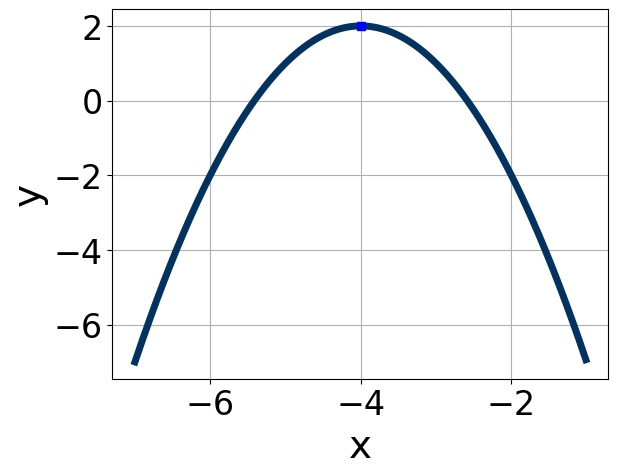
\includegraphics[width=0.5\textwidth]{../Figures/quadraticGraphToEquationC.png}
\end{center}
\begin{enumerate}[label=\Alph*.]
\item \( a \in [1, 4], \hspace*{5mm} b \in [-10, -6], \text{ and } \hspace*{5mm} c \in [15, 20] \)
\item \( a \in [-2, 0], \hspace*{5mm} b \in [7, 15], \text{ and } \hspace*{5mm} c \in [-16, -10] \)
\item \( a \in [-2, 0], \hspace*{5mm} b \in [7, 15], \text{ and } \hspace*{5mm} c \in [-19, -17] \)
\item \( a \in [1, 4], \hspace*{5mm} b \in [7, 15], \text{ and } \hspace*{5mm} c \in [15, 20] \)
\item \( a \in [-2, 0], \hspace*{5mm} b \in [-10, -6], \text{ and } \hspace*{5mm} c \in [-16, -10] \)

\end{enumerate} }
\end{enumerate}

\end{document}